\documentclass{article}
\usepackage[justification=raggedright, singlelinecheck=false]{caption}
\usepackage{graphicx}
\usepackage[margin=1in]{geometry}
\usepackage[doublespacing]{setspace}
\usepackage{subcaption}
  
\begin{document}
  \paragraph{name,matric} BN5205 Assignment 1 Question 2
  
  The Hodgkin-Huxley type model used in the paper is a system of ODEs. It is a 
  stiff system due to the interactions between the membrane potential $V$ and 
  the gating probabilities $n, h_t$ and $h_p$. The different activation 
  kinetics of the currents, fast activation in potassium current $I_K$ and 
  transient sodium current $I_{NaT}$ and slow activation in persistent sodium 
  current $I_{NaP}$, resulted in the sharp peak observed at around $t = 50 ms$, 
  this rapidly changing slope results in a stiff system (Fig. \ref{fig:peak}).
  \begin{figure}[h]
    \begin{subfigure}{.5\textwidth}
    \centering
    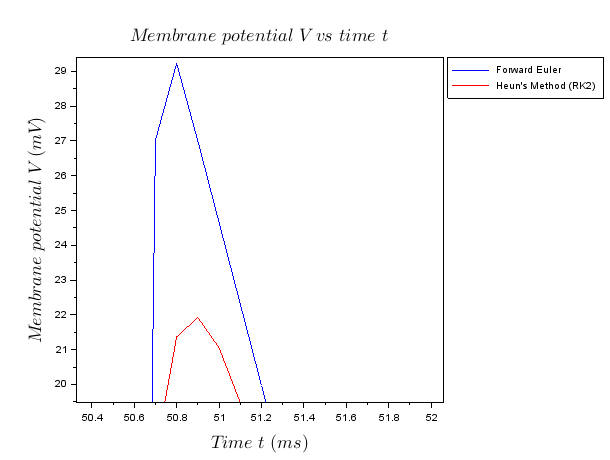
\includegraphics[width=230px]{img/large-tstep}
    \caption{ \label{fig:large-tstep}}
    \end{subfigure}
    \begin{subfigure}{.5\textwidth}
    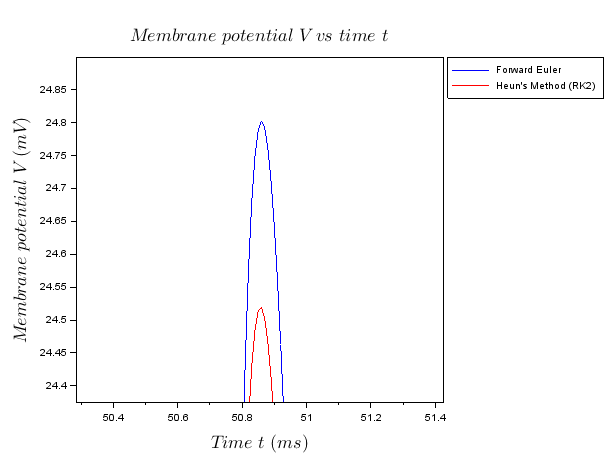
\includegraphics[width=230px]{img/small-tstep}
    \caption{ \label{fig:small-step}}
    \end{subfigure}
    \caption{\small Comparison of solution accuracy between large and small 
    time steps. Figures shown are close up view of the peaks of the solutions. 
    (a) $\Delta t$ = 0.1. (b) $\Delta t$ = 0.01. \label{fig:peak}}
  \end{figure}
  
  At a small time step of $\Delta t = 0.01$, the peak in membrane potential $V$ 
  computed by the Forward Euler method and Heun's Method are in close agreement 
  with each other. We assume the real solution lies between the peaks computed 
  by the two method, $V_{max} = 24.65 \pm 0.15 mV$ (Fig. \ref{fig:small-step}). 
  Therefore, we observed that the errors in estimation of the two methods 
  increase significantly when a larger time step $\Delta t = 0.1$ was used due 
  to the stiffness of the system (Fig. \ref{fig:large-tstep}).
\end{document}